\chapter{Introduction}\label{ch:introduction}
The basic approach of our project, just like any other based on embedded systems (\textit{microcontrollers}) largely depends on three main questions: 
\begin{itemize}
	\item Which microcontroller board would be appropriate?
	\item What \textit{sensor}(s) should be used to fulfill the goals of the project? 
	\item What actuators might be needed for introducing mechanical action, if needed? 
 
\end{itemize}

We had a literature survey through the internet about deciding the components needed for our project. This included studying in detail, several project ideas and instructions posted on blogs and YouTube.\\
We selected the following major components for having a \textsl{minimal}, \textsl{cost effective} and \textsl{efficient} apparatus that could do the job for us:
\begin{itemize}
	\item \textit{Microcontroller Board} - \arduinouno{}
	\item \textit{Sensor} - \hcsr{} \ultrasonic{}
	\item \textit{Actuator} - \servo{} Motor

\end{itemize}
The next few sections will explain the basis of selection of hardware for this project.

% r~\ref{ch:ch2label}.

\section{The \arduinouno}
\begin{figure}[H]
	\centering
	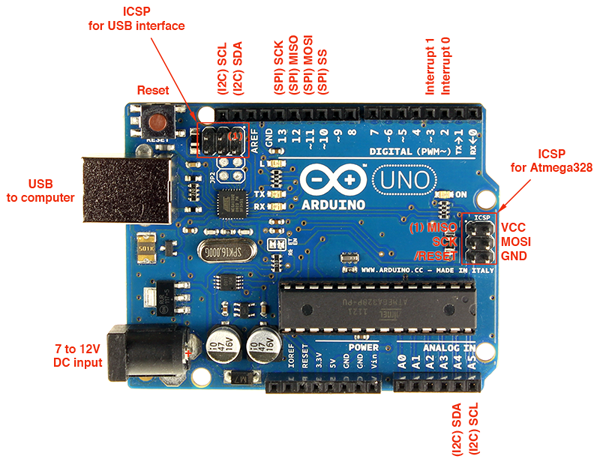
\includegraphics[width=0.5\textwidth]{../Files/ArduinoUno_R3_Pinouts_600}
	\caption{Arduino UNO Pinouts}  \label{fig:Arduino}
\end{figure}
Arduino is an open source electronics platform for fast prototyping of projects for users with minimal knowledge or experience in electronics and programming. We have used the \arduinouno, the most widely used variant of the Arduino.\\
Technically, Arduino Uno is a microcontroller board based on the 8-bit ATMega328P microcontroller. With 14 digital
input/output pins (including 6 PWM outputs), 6 analog inputs, a 16 MHz ceramic resonator, a USB connection, a power jack, an ICSP header, and a reset button, it has everything needed to support the microcontroller; we simply have to connect it to a computer with a USB cable or power it with a AC-to-DC adapter or battery to get started.\\
Arduino also comes with the Arduino IDE, in which we can write code and upload to the Arduino. The programming language used for an Arduino, called the Arduino Programming language, is very similar to C/C++ except that we can use inbuilt functions of the Arduino libraries which keep the code very simple and short.

\subsection{Why Arduino?}
We had the following reasons strongly backing our decision to choose the \arduinouno :
\paragraph{\textit{Support -}}
 Thanks to its simple and accessible user experience, Arduino has been used in thousands of different projects and applications. The Arduino software is easy-to-use for beginners, yet flexible enough for advanced users. It runs on Mac, Windows, and Linux.\\
 This has enabled a very large support base for Arduino, more than any other microcontroller board ever released in the market. Every problem/bug/question that we ever had throughout the course of this project was promptly answered by questions in online forums, as there was a very high probability that scores of people had already posted the same question and the issue was resolved by other experienced users.
 \paragraph{\textit{Cost Effective -}}
 The Arduino UNO, its basic variant that every beginner to embedded systems usually starts with, is available for less than \$25. Being an open source hardware and due to its simplicity, it is easily and widely replicable, which is also responsible for the growth of such a large community as mentioned in the earlier reason.
 \paragraph{\textit{Features -}} 
 \begin{table}
 \centering
 \begin{tabular}{|l|l|}
 	\hline
 	Microcontroller &ATmega328P(8-bit)\\
 	\hline
 	Operating Voltage &5V\\
 	\hline
 	Input Voltage  &(recommended) 7-12V; (limits) 6-20V\\
 	\hline
 	Digital I/O Pins &14 (of which 6 provide PWM output)\\
 	\hline
 	Analog Input Pins &6\\
 	\hline
 	DC Current per I/O Pin &40 mA\\
 	\hline
 	DC Current for 3.3V Pin &50 mA\\
 	\hline
 	Flash Memory &32 KB (ATmega328) of which 0.5 KB used by bootloader\\
 	\hline
 	SRAM &2 KB (ATmega328)\\
 	\hline
 	EEPROM &1 KB (ATmega328)\\
 	\hline
 	Clock Speed &16 MHz\\
 	\hline
 	Need of External Programmer &NO\\
 	\hline
 	Built-in LED &pin13\\
 	\hline
 	Length &68.6 mm\\
 	\hline
 	Width &53.4 mm\\
 	\hline
 	Weight &25 g\\
 	\hline
  \end{tabular}
  \caption{Features of Arduino UNO}
  \label{tab:FeaturesArduino}
\end{table}
 It is generally observed that the computing power and inbuilt memory of the Arduino easily supports a wide variety of circuits with multiple components along with continuous serial communication with another device/computer. Compared to the system configuration of the board, our project would require fairly low amount of resources. \vspace{0.1cm} \linebreak 
 The no. of GPIO pins on the UNO is more than sufficient considering the need for the circuitry in our project, as we shall see when we look at the pinouts of the servo motor and the sensor \-- the only two other devices being used in the project. \vspace{0.1cm} \linebreak
 One important advantage of using the UNO is that unlike most previous programmable circuit boards, the \textit{Arduino UNO does not need a separate piece of hardware (called a programmer) in order to load new code onto the board – we can simply use a USB cable.} The ATmega328 on the Arduino/Genuino Uno comes preprogrammed with a \textit{bootloader} that allows us to upload new code to it without the use of an external hardware programmer. \vspace{0.1cm} \linebreak
 Moreover, the components we have used work under the same operating voltage and current conditions as an arduino, especially considering the fact that such components are nowadays sold with their compatibility with arduino in mind.\\
 
 Considering the above factors, we found Arduino UNO to be the most appropriate microcontroller board to work with for this project.\\
 
\section{Examples}
You can also have examples in your document such as in example~\ref{ex:simple_example}.
\begin{example}{An Example of an Example}
  \label{ex:simple_example}
  Here is an example with some math
  \begin{equation}
    0 = \exp(i\pi)+1\ .
  \end{equation}
  You can adjust the colour and the line width in the {\tt macros.tex} file.
\end{example}


\subparagraph{A Subparagraph} Moreover, you can also use subparagraph titles which look like this\todo{Is it possible to add a subsubparagraph?}. They have a small indentation as opposed to the paragraph titles.

\todo[inline,color=green]{I think that a summary of this exciting chapter should be added.}

\section{The \hcsr \ultrasonic}
\begin{figure}[H]
	\centering
	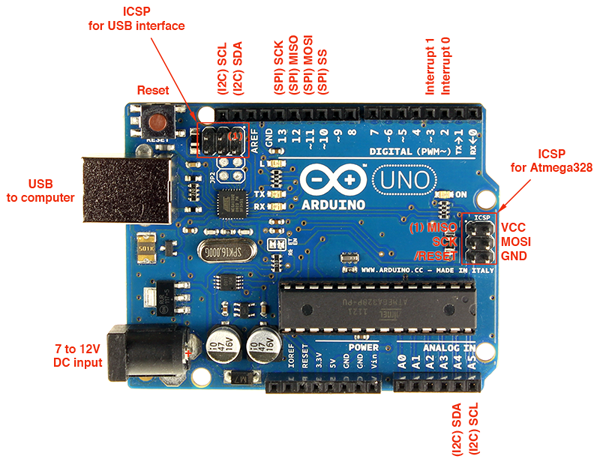
\includegraphics[width=0.5\textwidth]{../Files/ArduinoUno_R3_Pinouts_600}
	\caption{Arduino UNO Pinouts}  \label{fig:Arduino}
\end{figure}
Arduino is an open source electronics platform for fast prototyping of projects for users with minimal knowledge or experience in electronics and programming. We have used the \arduinouno, the most widely used variant of the Arduino.\\
Technically, Arduino Uno is a microcontroller board based on the 8-bit ATMega328P microcontroller. With 14 digital
input/output pins (including 6 PWM outputs), 6 analog inputs, a 16 MHz ceramic resonator, a USB connection, a power jack, an ICSP header, and a reset button, it has everything needed to support the microcontroller; we simply have to connect it to a computer with a USB cable or power it with a AC-to-DC adapter or battery to get started.\\
Arduino also comes with the Arduino IDE, in which we can write code and upload to the Arduino. The programming language used for an Arduino, called the Arduino Programming language, is very similar to C/C++ except that we can use inbuilt functions of the Arduino libraries which keep the code very simple and short.

\subsection{Why Arduino?}
We had the following reasons strongly backing our decision to choose the \arduinouno :
\paragraph{\textit{Support -}}
Thanks to its simple and accessible user experience, Arduino has been used in thousands of different projects and applications. The Arduino software is easy-to-use for beginners, yet flexible enough for advanced users. It runs on Mac, Windows, and Linux.\\
This has enabled a very large support base for Arduino, more than any other microcontroller board ever released in the market. Every problem/bug/question that we ever had throughout the course of this project was promptly answered by questions in online forums, as there was a very high probability that scores of people had already posted the same question and the issue was resolved by other experienced users.
\paragraph{\textit{Cost Effective -}}
The Arduino UNO, its basic variant that every beginner to embedded systems usually starts with, is available for less than \$25. Being an open source hardware and due to its simplicity, it is easily and widely replicable, which is also responsible for the growth of such a large community as mentioned in the earlier reason.
\paragraph{\textit{Features -}} 
\begin{table}
	\centering
	\begin{tabular}{|l|l|}
		\hline
		Microcontroller &ATmega328P(8-bit)\\
		\hline
		Operating Voltage &5V\\
		\hline
		Input Voltage  &(recommended) 7-12V; (limits) 6-20V\\
		\hline
		Digital I/O Pins &14 (of which 6 provide PWM output)\\
		\hline
		Analog Input Pins &6\\
		\hline
		DC Current per I/O Pin &40 mA\\
		\hline
		DC Current for 3.3V Pin &50 mA\\
		\hline
		Flash Memory &32 KB (ATmega328) of which 0.5 KB used by bootloader\\
		\hline
		SRAM &2 KB (ATmega328)\\
		\hline
		EEPROM &1 KB (ATmega328)\\
		\hline
		Clock Speed &16 MHz\\
		\hline
		Need of External Programmer &NO\\
		\hline
		Built-in LED &pin13\\
		\hline
		Length &68.6 mm\\
		\hline
		Width &53.4 mm\\
		\hline
		Weight &25 g\\
		\hline
	\end{tabular}
	\caption{Features of Arduino UNO}
	\label{tab:FeaturesArduino}
\end{table}
It is generally observed that the computing power and inbuilt memory of the Arduino easily supports a wide variety of circuits with multiple components along with continuous serial communication with another device/computer. Compared to the system configuration of the board, our project would require fairly low amount of resources. \vspace{0.1cm} \linebreak 
The no. of GPIO pins on the UNO is more than sufficient considering the need for the circuitry in our project, as we shall see when we look at the pinouts of the servo motor and the sensor \-- the only two other devices being used in the project. \vspace{0.1cm} \linebreak
One important advantage of using the UNO is that unlike most previous programmable circuit boards, the \textit{Arduino UNO does not need a separate piece of hardware (called a programmer) in order to load new code onto the board – we can simply use a USB cable.} The ATmega328 on the Arduino/Genuino Uno comes preprogrammed with a \textit{bootloader} that allows us to upload new code to it without the use of an external hardware programmer. \vspace{0.1cm} \linebreak
Moreover, the components we have used work under the same operating voltage and current conditions as an arduino, especially considering the fact that such components are nowadays sold with their compatibility with arduino in mind.\\

Considering the above factors, we found Arduino UNO to be the most appropriate microcontroller board to work with for this project.\\

\section{Examples}
You can also have examples in your document such as in example~\ref{ex:simple_example}.
\begin{example}{An Example of an Example}
	\label{ex:simple_example}
	Here is an example with some math
	\begin{equation}
	0 = \exp(i\pi)+1\ .
	\end{equation}
	You can adjust the colour and the line width in the {\tt macros.tex} file.
\end{example}


\subparagraph{A Subparagraph} Moreover, you can also use subparagraph titles which look like this\todo{Is it possible to add a subsubparagraph?}. They have a small indentation as opposed to the paragraph titles.

\todo[inline,color=green]{I think that a summary of this exciting chapter should be added.}
